\begin{figure}\center%
  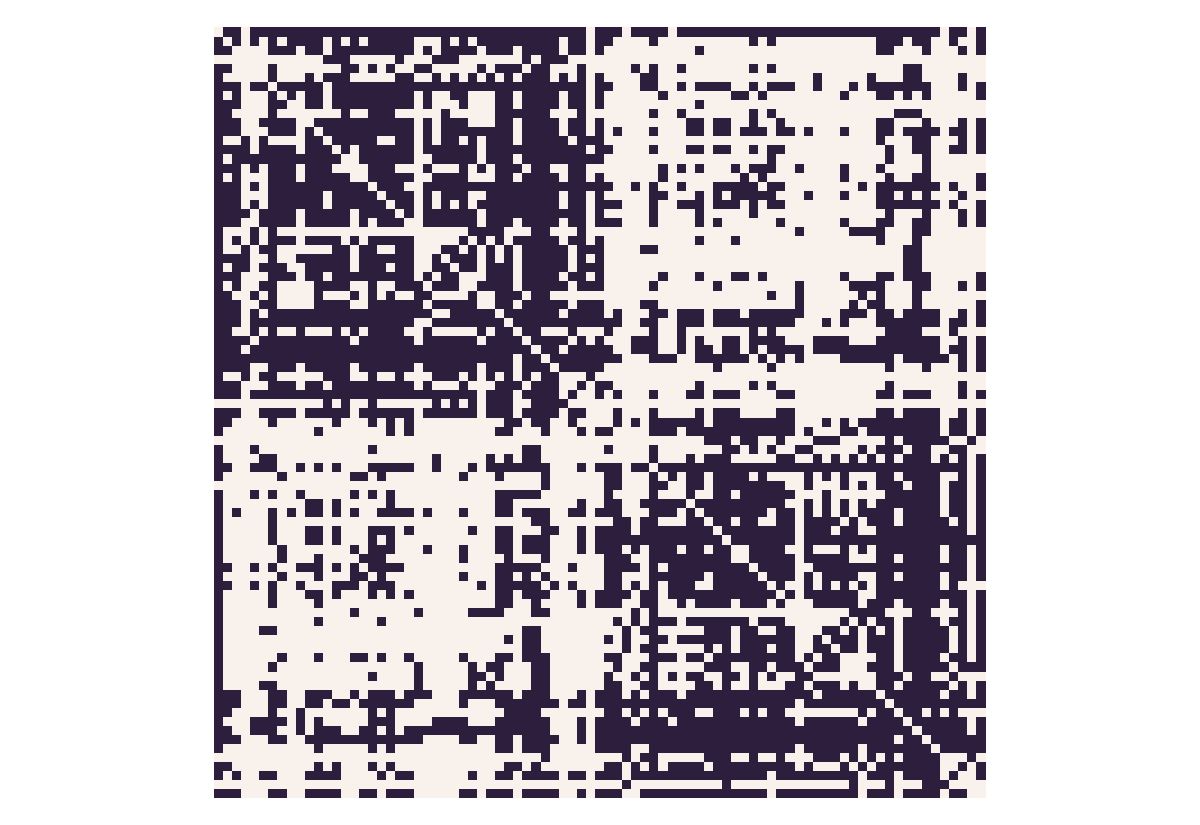
\includegraphics[height=.15\textheight]{connectome-5}
  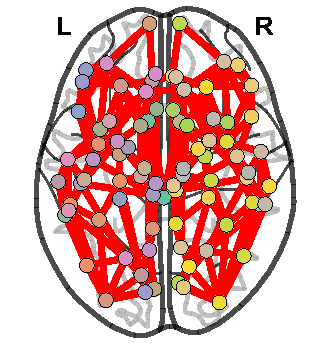
\includegraphics[height=.15\textheight]{connectome-9}
  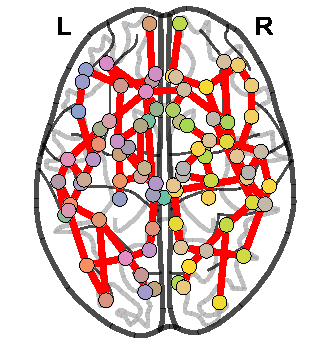
\includegraphics[height=.15\textheight]{connectome-99}
  \caption{Core structural connectivity network computed by our approach. On the left, we show the adjacency matrix for $\lambda = 0.5$, where 48.19\% of the connections were included in the CSCN. In the central and right panels, we show the resulting CSCN for $\lambda=0.9$ and $0.99$ respectively. The percentage of included connections in the CSCN is 5.99\% and 1.27\% respectively.\label{fig:connectome}}
  
\end{figure}

We formalized the CSCN problem in section \ref{problem_section} and designed an algorithm to solve it in section \ref{heuristic}. Now we will asses the performance of our method. For this, we compare it with the most used~\cite{Gong2009} and with the recent one~\cite{Wassermann2016} in the task of connectivity prediction performance.

We use a subset of the HCP500 dataset~\cite{Sotiropoulos2013}: all subjects aged 21-40 with complete dMRI protocol, totaling 309. We compute the weighted connectivity matrices between the cortical regions defined by the Desikan atlas~\cite{Desikan2006} as done by Sotiropoulos et al.~\cite{Sotiropoulos2013}.
Examples of CSCN exctracted with our algorithm at different $\lambda$ levels are shown in Fig.~\ref{fig:connectome}, which was generated using Nilearn~\cite{Abraham2014}.

\subsection{Consistency of the Extracted Graph}
To compare the stability across different algorithms for CSCN, we use an analysis based on Wassermann et al.~\cite{Wassermann2016}: we randomly take $500$ subsets of $100$ subjects each and computed the core graphs for all subsets. We then compute the number of \emph{unstable connections}: connections that present in at least one core graph but not in all of them. Finally, in Table~\ref{table:number_of_features} we report each algorithm's \emph{stability}: 

$$\text{stability of the algorithm} \triangleq 1 - \frac{\#\{\text{unstable connections}\}}{\#\{\text{total connections}\}}~.$$

This measure quantifies the CSCN consistency across subsamples. Due to the homogeneity of our sample, we expect the CSCNs obtained by an algorithm to be similar across subsamples. Hence, a stabler algorithm is preferable.

%\todo{You need to explain how to measure stability here and to the refer it to the Table. You need to add to the discussion what conclusions you can drive from the stability study}

\subsection{Predicting Handedness-Specific Connectivity}

We evaluate performance of the methods by using the generated core graphs as a feature selection for handedness specific connectivity. We use a nested Leave-$\tfrac 1 3$-Out procedure: the outer loop performs model selection on $\tfrac 1 3$ of the subjects using the core graph algorithm and the inner loop performs model fitting and prediction using the selected features.

\begin{table}
\centering

\caption{Stability of the algorithms and amount of features selected by linear regression in the core graph relating the weights with handedness. Our procedure gets more features selected than Gong et al.~\cite{Gong2009} and Wassermann et al.~\cite{Wassermann2016}, showing better statistical power. It's also more stable than Gong et al., showing improved consistency. \label{table:number_of_features}}
\begin{tabular}{ l c c c }
	\hline
    Algorithm & Features (mean) & Features (std) & Stability \\
    \hline
    Gong et al. 2009& 0.066 & 0.256 & 0.364 \\
    %\hline
    Wassermann et al. 2016 & 0.415 & 0.723 & 0.644 \\
    %\hline
    Our approach ($\lambda = 0.50$) & 1.042 & 1.269 & 0.528 \\
    %\hline
\end{tabular}
\end{table}


%\begin{figure}\center%
%  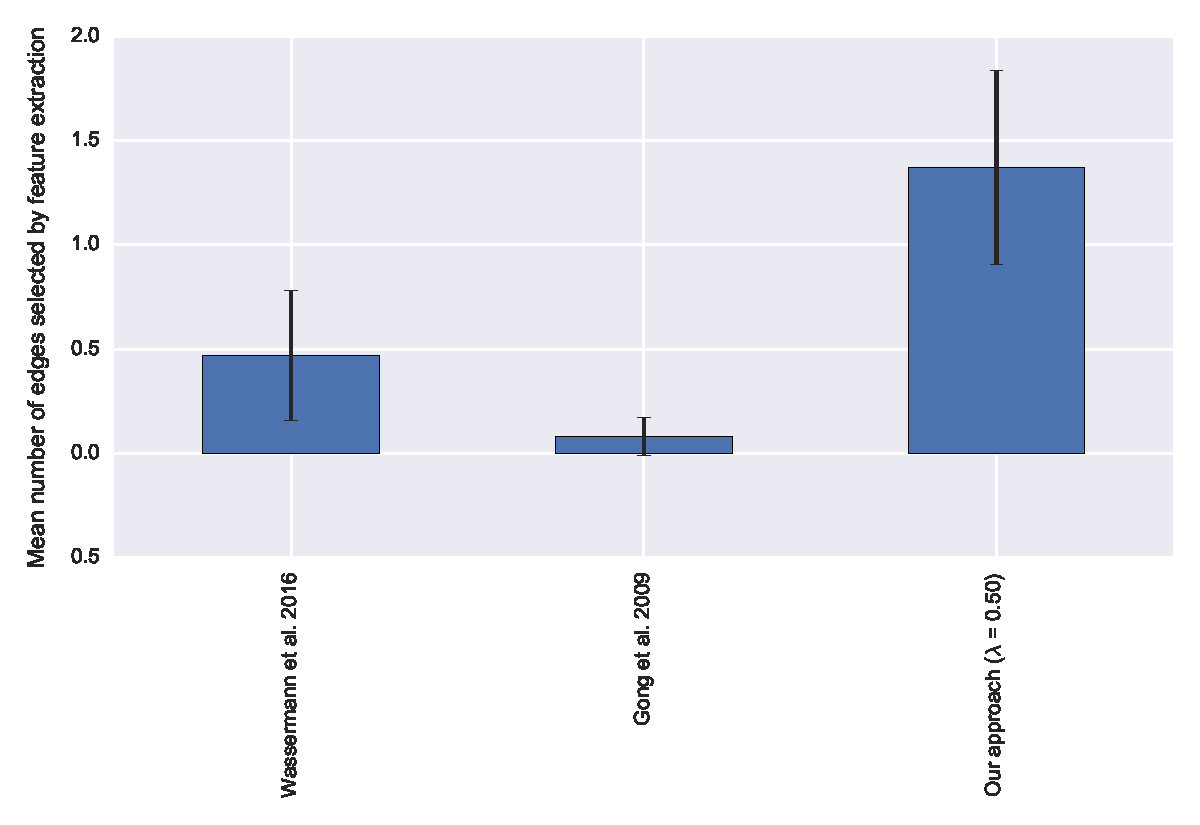
\includegraphics[height=.4\textheight]{number_of_features}
%  \caption{Amount of features selected by linear regression in the core graph related to handedness. Our procedure gets more features selected than Gong~\cite{Gong2009} and Wassermann~\cite{Wassermann2016}, showing better statistical power.\label{fig:number_of_features}}
%\end{figure}
\begin{figure}\center%
  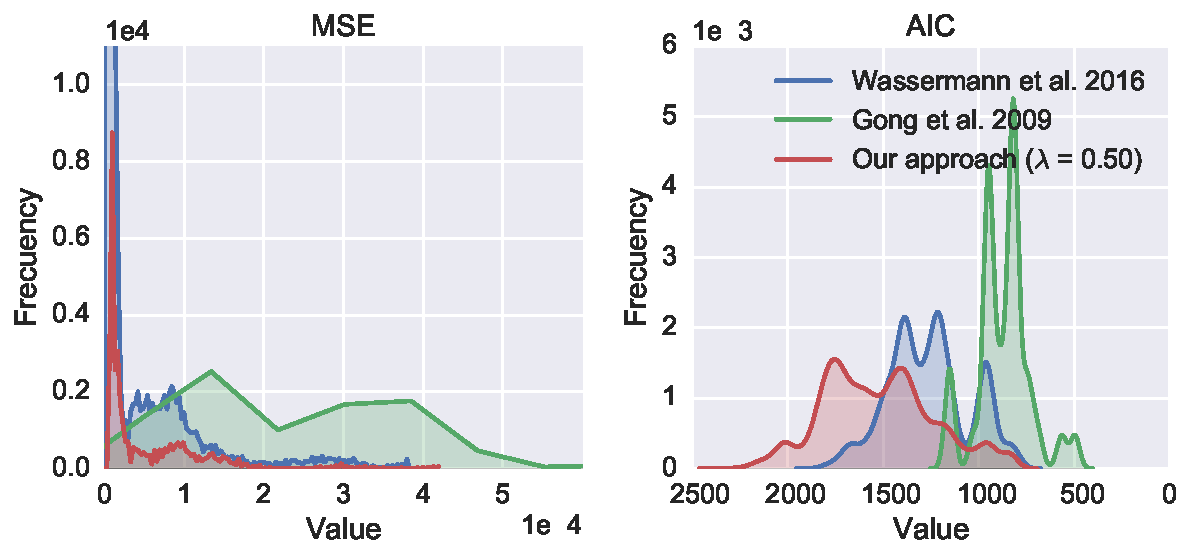
\includegraphics[height=.3\textheight]{prediction_performance}
  \caption{Performance of core network as feature selection for a linear model for handedness specific connectivity. We evaluate model prediction (left) and fit (right) for Gong et al.~\cite{Gong2009} in green, Wassermann et al.~\cite{Wassermann2016} in blue and ours, in red. We show the histograms from our nested Leave-$\tfrac 1 3$-Out experiment. In both measures, our approach has more frequent lower values than Gong et al., showing a better performance.\label{fig:prediction_performance}}
\end{figure}

Specifically, we first take $\tfrac 1 3$ subjects randomly and compute the core graph for those subjects using the three different algorithms. Then we add the weights for the selected edges for each subject, and select the features $F$ that are more determinant of handedness using a linear least-squares regression and the Bonferroni correction for multiple hypotheses. This experiment is repeated 500 times. We quantify the amount of features that are selected after each procedure, which indicates how useful is the core graph algorithm for selecting the edges related to handedness. % We also evaluate the stability of the methods by counting the proportion of edges that are nor present or absent in all core graphs.
We show the results in Table~\ref{table:number_of_features}.

To evaluate the prediction, we randomly take $\tfrac 1 2$ of the remaining subjects and fit a linear model on the features $F$ to predict connectivity weights using the handedness of each subject. Finally, we predict the values of the features $F$ from the handedness in the subjects left out. We quantify the quality of the linear model fitting Akaike Information Criterion (AIC) and of the prediction performance with the mean squared error (MSE) of the prediction. For both measures a lower value indicates better performance. The outer loop is performed 500 times and the inner loop 100 times per outer loop, which totals 50,000 experiments. We show the results of this experiments in Fig.~\ref{fig:prediction_performance}.

